\section{Optimising Abstract Graph Size}
\par \indent
As we have observed in lemmas \ref{aha-lemma:maxedgesincluster} and \ref{aha-lemma:maxtransitions} the initial abstraction algorithm attempts to represent every optimal path between clusters and inside clusters. However, while studying this problem we were unable to concot any scenarios where the number of edges is equal to the the theoretical worst-case suggesting that it is, infact, a mere approximation (or a highly pathological case).  A more exact characterisation is not easily derived due mostly to the combinatorial blow-up of possible terrain arrangements on even small maps with highly limited variable domains.
\par \indent 
A consequence of this observation is that in all experimental scenarios the same path was often returned for different pairs of $(c, s)$ parameters when using AA* to discover intra-edges. We highlight the problem in figure \ref{aha-fig:strongdominance}(a) and contrast it with our desired result in \ref{aha-fig:strongdominance}(b). $\lbrace E3, E5 \rbrace$ represent the same path between nodes $b$ and $c$ but are annotated with different clearance values. The same problem is evident for $\lbrace E4, E6 \rbrace$ which both cover nodes $a$ and $c$. In such cases we say that $E3$ and $E4$ are \emph{strongly dominant}, which we denote $E3 \prec E5$ and $E4 \prec E6$. We give the following theorem to formalise this concept:

\begin{theorem}
\label{aha-theorem:strongdominance}
$e_{1} \prec e_{2}$ iff  $e_{1}(c) \geq e_{2}(c) \wedge weight(e_{1}) \leq weight(e_{2})$.
\end{theorem}

We term the resultant graph in which all strongly dominant edges have been removed a \emph{high-quality} abstraction. In figure \ref{aha-fig:abstractgraph}(c) we can see the complete graph for our running example; we were able to represent a 2-terrain map with 100 nodes and 350 edges using just 13 nodes and  22 edges. 

\begin{figure}[htbp]
        \caption{\emph{Strong edge dominance} }
        \begin{center}
                        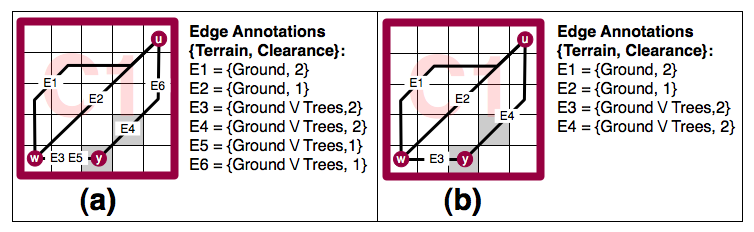
\includegraphics[scale=0.3]{diagrams/intraedges_initial.png}
        \end{center}
        \label{aha-fig:strongdominance}
\end{figure}

The abstract graph can be further reduced by noticing that some multi-terrain transitions between clusters can be removed without affecting the completeness of the representation. 
Figure \ref{aha-fig:abstractgraph}(a) highlights the problem and \ref{aha-fig:abstractgraph}(b) the desired outcome.
In this example we can see that edges $E5$ and $E6$ have the same clearance but are traversable by different capabilities. 
However, any agent capable of traversing $E6$ can also traverse $E5$ without loss of generality. 
We may further notice that the same is also true for $E7$ which suggests we can remove both $E6$ and $E7$ without losing any connectivity information from the graph. 
In such cases we say $E5$ is \emph{weakly dominant} and denote it as $E5 \sim E6$ and $E5 \sim E7$. 
We formalise the concept using the following theorem:
\begin{theorem}
\label{aha-theorem:weakdominance}
Let $(n1_{a}, n2_{a}), (n1_{b}, n2_{b}) \in V_{abs}$ denote two pairs of abstract nodes in two adjacent clusters $\lbrace L_{1}, L_{2} \rbrace$ each covered covered by an inter edge $e_{a}, e_{b} \in E_{abs}$ with clearance values $e_{a}(c_{a}), e_{b}(c_{b})  : c_{a}, c_{b} \in C$.
 In this scenario, $e_{a} \sim e_{b}$ iff the following conditions are met:
\begin{enumerate}
\item{The capability dominance condition: $e_{a}(c_{b}) \geq e_{b}(c_{b})$}
\item{The circuit condition: $\exists intra_{1}, intra_{2} \in E_{abs} : (n1_{a}, n1_{b}) \in intra_{1} \wedge (n2_{a}, n2_{b}) \in intra_{2} \wedge intra_{1}(c_{b}) \geq e_{b}(c_{b}) \wedge intra_{2}(c_{b}) \geq e_{b}(c_{b})$.}
\end{enumerate}
Then, any location which an agent can reached by traversing $e_{b}$ can also be reached by $e_{a}$.
\end{theorem} 

\begin{proof}
If a circuit exists between the endpoints $\lbrace n1_{a}, n2_{a}, n1_{b}, n2_{b} \rbrace$ which contains only edges with clearances at least as large as $e_{b}(c_{b})$ for the capability $c_{b}$ then any nodes which are reachable from $n1_{b}$ or $n2_{b}$ are also reachable from $n1_{a}$ or $n2_{a}$.
From this it follows that any destination an agent can reach via $e_{b}$ can also be reached via $e_{a}$ \qed
\end{proof}
In addition to removing weakly dominated edges, we can also remove their endpoints, provided they do not connect any other inter-edges. We thus refer to the initial abstraction that has had both strong and weakly dominated edges removed a \emph{low quality abstraction}.
In \ref{aha-fig:abstractgraph}(d) we show a low-quality abstraction. 
In this trival example we reduce the high quality abstraction from \ref{aha-fig:abstractgraph}(c) to 10 nodes and 11 edges.
\begin{figure}[htbp]
        \caption{\emph{High and low quality abstraction results} }
        \begin{center}
                        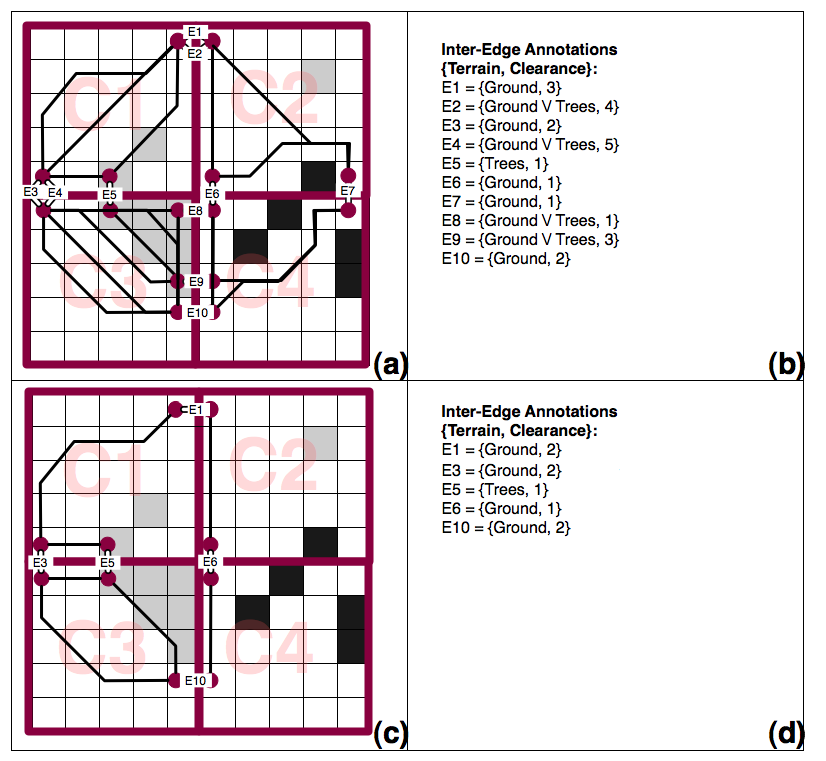
\includegraphics[scale=0.25]{diagrams/abstraction_result.png}
        \end{center}
        \label{aha-fig:abstractgraph}
\end{figure}
\par \indent
A reasonable analogy to highlight the intuition behind theorem \ref{aha-theorem:weakdominance} is to compare the way off-road vehicles opportunistically use roads where possible even if an off-road route (or trail) might exist which has a smaller distance cost. Roads are smoother to drive on and have other benefits such less wear and tear, and better fuel consumption. Opting for a lower-quality abstraction in this way does have an effect on the quality of the computed solutions, but as we will show, the differences are reasonably small and the solutions still near-optimal. The best choice depends on the requirements of the specific application to which the algorithm is applied; it is a classic tradeoff between performance vs space.
\par \indent


